%   % !TEX root = ../../VIII,3_Rahmen-TeX_9-0.tex
%  
%   Band VIII, 3 N.~?? 	[XXX??.?]			(Unter)rubrik			??
%   Signatur/Tex-Datei:	LH_37_05_155-156
%   RK-Nr. 	60345		
%				
%   Überschrift: 	(keine)
%   Titel: 			??			(unser Titel)					??
%   Datierung:		???? bis ???? (a. St.?), eigh. (?)				??
%   Textfolge: 					(ggf. wie Foliierung)				??
%   WZ: 	im Falz, Nr. 803022
%   edlabels:			11
%   Diagramme: 		5 (+ 1 gestr. + 1 Vorstufe)
%   Dateien (PDF):
%   		LH_37_05_155-156_d1_155r;
%   		LH_37_05_155-156_d2_155r;
%   		LH_37_05_155-156_d3_155v;
%   		LH_37_05_155-156_d4_155v;
%   		LH_37_05_155-156_d5_155v;
%   		LH_37_05_155-156_d6_156r
%
%
%   Erstaufnahme:			(wer?)
%   Bearbeitung MS ab: 		August 2020
%
%   NB: 						(Anmerkungen)					??
%
%
%
\selectlanguage{ngerman}
\frenchspacing
%
\begin{ledgroupsized}[r]{120mm}
\footnotesize
\pstart
\noindent\textbf{Überlieferung:}
\pend
\end{ledgroupsized}
%
\begin{ledgroupsized}[r]{114mm}
\footnotesize
\pstart \parindent -6mm
\makebox[6mm][l]{\textit{L}}%
Konzept:
LH~XXXVII~5, Bl.~155\textendash156. 
Ein Bogen~4\textsuperscript{o};
Wasserzeichen im Falz;
Papiererhaltungsmaßnahmen;
Ränder beschnitten.
Vier Seiten.
\pend
\end{ledgroupsized}
%
%
\vspace{5mm}
\begin{ledgroup}
\footnotesize
\pstart
\noindent%
\textbf{Datierungsgründe:} %%
N.~\ref{RK60345} zeugt von Leibnizens Kenntnis des auf dem Relativitätsprinzip (bzw.\ der \glqq compositio motuum\grqq) beruhenden 
%
Schiffsmodells zur Stoßanalyse, die er in den
%
eigh.\ auf den 10.\ und 11.\ (20.\ und 21.) Juni 1677 datierten Konzepten N.~\ref{RK57269}\textendash\ref{RK57271} ausführlich besprochen hatte.
%
Hier bezeichnet er diese Methode als  \glqq ratiocinatio per compositionem motuum\grqq\
und wendet sie mehrmals an, um von einfacheren, bekannten Konfigurationen des geraden Stoßes zweier Körper auf komplexere überzugehen
(siehe S.~\refpassage{37_05_155-156_10a}{37_05_155-156_10b}, S.~\refpassage{37_05_155-156_11a}{37_05_155-156_11b}).
%
Daher kann man von einer Entstehung von N.~\ref{RK60345} nach den obengenannten Konzepten ausgehen.
%
Dass im Übrigen das Wasserzeichen auch bei zwei dieser Konzepte (N.~\ref{RK57270} und N.~\ref{RK57269}) belegt ist,
%
lässt die Vermutung einer Entstehung von N.~\ref{RK60345} kurz nach diesen Stücken zu.
\pend
%
\pstart
Die Vermutung wird bekräftigt durch den Umstand,
%
dass Leibniz sich in N.~\ref{RK60345} mit der These der \glqq permutatio potentiarum\grqq\ zweier Körper beim Stoß beschäftigt,
%
einer mit den klassischen Stoßregeln inkompatiblen Annahme,
%
die bereits in N.~\ref{RK57268} (Mai 1677) und in N.~\ref{RK57274} (wohl Mai bis Mitte Juni 1677) eine wichtige Rolle gespielt hatte (siehe die Datierungsgründe).
%
Im ersteren dieser Stücke war sie eine tragende Prämisse der Beweisführung, der Leibniz ohne Einschränkung zustimmte.
%
In N.~\ref{RK57274} hielt er sie noch für ein \glqq theorema universalissimum\grqq\ und eine Wahrheit, die aus metaphysischen Prinzipien der Natur fließt (S.~\refpassage{37_05_150-151_6a}{37_05_150-151_6b});
%
wobei er angesichts der Tatsache, dass in den meisten empirisch beobachtbaren Stoßvorgängen die Körper ihre Bewegungsgrößen nicht austauschen, die Geltung der These auf unelastische Körper eingeschränkt
%
und für die davon abweichenden Phänomene die Elastizität der Körper
%
verantwortlich gemacht hatte.
%
In N.~\ref{RK57271} vom 11.\ (21.) Juni 1677 kam Leibniz zum Schluss, dass die These zu verwerfen sei:
%
\glqq ergo haec regula falsa est, ex qua sequeretur semper permutari potentias\grqq\ (S.~\refpassage{37_05_159-160_13a}{37_05_159-160_13b}).
%
Im vorliegenden Konzept legt Leibniz eine gewisse Unsicherheit hinsichtlich der \glqq permutatio potentiarum\grqq\ an den Tag:
%
Teils nimmt er die These für wahr an, oder versucht sich an einem Beweis auf der Basis der beiden Grundregeln des Stoßes
%
(S.~\refpassage{37_05_155-156_7a}{37_05_155-156_7b}), was dem Verfahren von N.~\ref{RK57274} entspricht;
%
teils bemerkt er, dass aus der \glqq permutatio potentiarum\grqq\ absurde bzw.\ mit seiner \glqq ratiocinatio per compositionem motuum\grqq\
%
unvereinbare Folgen fließen müssten (S.~\refpassage{37_05_155-156_8a}{37_05_155-156_8b}), weshalb er die These wie in N.~\ref{RK57271} ablehnt.
%
Das Fehlen einer konsequent ausgearbeiteten Position und Leibnizens Schwanken zwischen den geschilderten Optionen lässt
%
die Vermutung einer Entstehung von N.~\ref{RK60345} kurze Zeit nach den Konzepten vom 20.\ und 21. Juni, also wohl im Sommer 1677, plausibel erscheinen.
\pend


%
\end{ledgroup}
%
%
\selectlanguage{latin}
\frenchspacing
% \newpage%
\vspace{8mm}
\pstart%
\normalsize%
\noindent%
\lbrack155~r\textsuperscript{o}\rbrack\
%
Videndum an hac liceat uti regula, quod eadem potentia\protect\index{Sachverzeichnis}{potentia} eundem in eandem potentiam\protect\index{Sachverzeichnis}{potentia} producat effectum.\protect\index{Sachverzeichnis}{effectus} \pend
% 
%
\vspace{1.0em} %%%%%%%%% Diagramm 1
\centerline{%
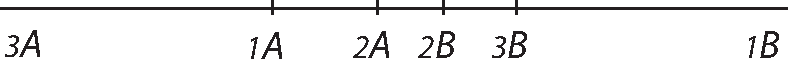
\includegraphics[width=0.55\textwidth]{%
gesamttex/edit_VIII,3/images/LH_37_05_155-156_d1_155r.pdf%
}} 
\vspace{0.2em}
\centerline{%
\lbrack\textit{Fig.~1}\rbrack%
}
% \newpage%
\vspace{1em}
%
%
\pstart 
%
\edtext{Duo corpora %
%
\edtext{aequalia\protect\index{Sachverzeichnis}{corpora aequalia} sibi occurrunt,}{\lemma{aequalia}\Bfootnote{\textit{(1)}~concurrunt, \textit{(2)}~sibi occurrunt,~\textit{L}}}
%
post occursum\protect\index{Sachverzeichnis}{occursus} feruntur reciprocis celeritatibus,\protect\index{Sachverzeichnis}{celeritates reciprocae} quemadmodum demonstratum est.}{%
\lemma{Duo \lbrack...\rbrack\ demonstratum est}%
\Cfootnote{%
Siehe bspw.\ N.~\ref{RK57268} von Mai 1677.}}
%
Ergo%
\edlabel{37_05_155-156_1a}%
\edtext{}%
{{\xxref{37_05_155-156_1a}{37_05_155-156_1b}}%
\lemma{Ergo}%
\Bfootnote{\textit{(1)}~si potentia erit \textit{(2)}~si~\textit{L}}}
%
\pend
%
\pstart\noindent
\begin{tabular}[t]{rcc} 
si\edlabel{37_05_155-156_1b} corpora&\textit{a}&\textit{b}\\
celeritates priores&\textit{e}&\textit{f}\\
posteriores&\textit{i}&\textit{m}\\
\end{tabular}
%
erunt $i \sqcap f$. et $m \sqcap e$.%
\pend
%
\pstart
Potentia\protect\index{Sachverzeichnis}{potentia agens}
%
agens erat
%
\begin{tabular}[t]{c}
\textit{ae},\\
\textit{bf}\\ 
\end{tabular} effectus\protect\index{Sachverzeichnis}{effectus} in patiente\protect\index{Sachverzeichnis}{patiens}
%
\edlabel{37_05_155-156_3a}%
\edtext{}{% B-Footnote Tabelle ae, bf
{\xxref%
{37_05_155-156_3a}{37_05_155-156_3b}}%
\lemma{}%
\Bfootnote{%
$\protect\underset%
{\displaystyle \textit{bf}\protect\phantom{I}}% Unten
{\textit{ae},\protect\vphantom{j}}$ % Mittig
\textit{L ändert Hrsg.}%
}}%
\begin{tabular}[t]{c}
\lbrack\textit{ai}\rbrack,\\
\lbrack\textit{bm}\rbrack.\\ 
\end{tabular}
\edlabel{37_05_155-156_3b}
%
\pend
%
\vspace{1.0em} %%%%%%%%% Diagramm 2
\centerline{%
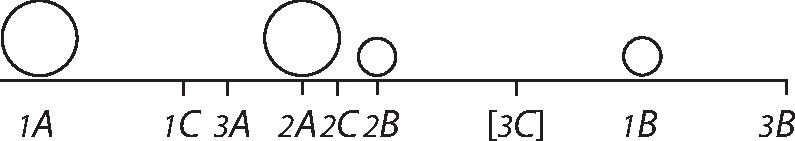
\includegraphics[width=0.6\textwidth]{%
gesamttex/edit_VIII,3/images/LH_37_05_155-156_d2_155r.pdf%
}} 
\vspace{0.5em}
\centerline{%
\lbrack\textit{Fig.~2}\rbrack%
}
% \newpage%
\vspace{1em}
%
\pstart 
%
\hspace{1mm}\hspace{-1mm}% Trick, weil \edlabel nicht zu \par-Beginn sein darf
\edlabel{37_05_155-156_8a}%
%
\edtext{Sint}{%		% TRICK für Fig. 2
\lemma{\hspace*{1,6mm}%
\lbrack\textit{Fig.~2}\rbrack%
}\killnumber%
\Cfootnote{%
Die Bezeichnung für Punkt \textit{{\scriptsize3}C} ergänzt Hrsg.%
}}
%
jam corpora inaequalia\protect\index{Sachverzeichnis}{corpora inaequalia} celeritas vero aequalis, videntur post concursum\protect\index{Sachverzeichnis}{concursus} %
%
\edtext{debere esse celeritates tales ut}%
{\lemma{debere}%
\Bfootnote{\textit{(1)}~permutari \textit{(2)}~celeritates esse 
\textit{(3)}~esse celeritates
\textit{(a)}~in corporum ratione reciproca, 
\textit{(aa)}~ut scilicet 
\textit{(bb)}~. Nimirum 
\textit{(b)}~tales ut~\textit{L}}}
%
vires\protect\index{Sachverzeichnis}{vis} permutentur.\protect\index{Sachverzeichnis}{permutatio virium}
%
\pend
%
\pstart\noindent
%
\rule[0cm]{0mm}{16pt}$ae \sqcap bm$.  $bf \sqcap ai$.  $\displaystyle\frac{ae}{ai} \sqcap \displaystyle\frac{bm}{bf}$.  $\displaystyle\frac{e}{i} \sqcap \displaystyle\frac{m}{f}$.
$m \sqcap \displaystyle\frac{ae}{b}$.  $i \sqcap \displaystyle\frac{bf}{a}$.
%
\pend
%
\pstart\noindent
\rule[0cm]{0mm}{10pt}Sed hoc absurdum esse inde colligo, quia hoc modo corpus quantumcunque a parvo utcunque repelletur.\edlabel{37_05_155-156_8b}
\pend
% %
\pstart 
Videndum an hac regula uti
%
\edlabel{37_05_155-156_2a}%
\edtext{}{% 
{\xxref%
{37_05_155-156_2a}{37_05_155-156_2b}}%
\lemma{liceat.}%
\Bfootnote{%
\textit{(1)}~Si corpus \textit{a} celeritate \textit{e} \textit{(2)}~Faciat corpus \textit{(3)}~Sit~\textit{L}}}%
liceat.
\pend
%
\pstart
Sit%
\edlabel{37_05_155-156_2b}
%
%
\begin{tabular}[t]{ccc}
\textit{a}&\textit{e}&\textit{i}\\
\textit{b}&\textit{f}&\textit{m}\\
\end{tabular}
et
\begin{tabular}[t]{ccc}
$\alpha$&$\epsilon$&$\upsilon$\\
$\beta$&$\phi$&$\mu$\\
\end{tabular} 
sitque
\begin{tabular}[t]{c}
$\alpha\epsilon \sqcap ae$\\
$\beta\phi \sqcap bf$\\
\end{tabular}.
%
Erit
\begin{tabular}[t]{c}
$ai \sqcap \alpha\upsilon$\\
$bm \sqcap \beta\mu$\\
\end{tabular}. 
%
%
\edlabel{37_05_155-156_4a}%
\edtext{}{% C-Footnote Fehler im Argument
{\xxref%
{37_05_155-156_4a}{37_05_155-156_4b}}%
\lemma{Ponamus \lbrack...\rbrack\ progredietur}%
\Cfootnote{%
Leibniz hat die Gleichung $\displaystyle\frac{\upsilon}{\epsilon} \sqcap \displaystyle\frac{\phi}{\mu}$
zwar korrekt hergeleitet, aber unter ihren Prämissen ist die Setzung $a \sqcap b$.
Diese entspricht der Annahme, dass die Körper \textit{a} und \textit{b} gleiche Massen haben.
Daraus folgt, dass auch $\alpha$ und $\beta$ gleiche Masse haben müssen:
Die Formel $\displaystyle\frac{\upsilon}{\epsilon} \sqcap \displaystyle\frac{\phi}{\mu}$ gilt nur unter dieser Einschränkung und kann daher nicht auf den Stoß unter Körpern beliebiger Masse 
(\textit{corpus utcunque magnum} bzw.\ \textit{utcunque parvum})
erweitert werden.}}%
%
Ponamus ergo 
%
\rule[0cm]{0mm}{10pt}$a \sqcap b$. erit $i \sqcap f$. et $m \sqcap e$. ergo $ai \sqcap af$. et $bm \sqcap ae$. %
%
%
\pend
%
\pstart\noindent
\edtext{Jam quia}{\lemma{Jam}\Bfootnote{\textit{(1)}~sit \textit{(2)}~quia~\textit{L}}}
%
 $\alpha\upsilon \sqcap ai$, erit $\alpha\upsilon \sqcap af$ 
 %
\edtext{et quia $\beta\mu \sqcap bm$,}{\lemma{}\Bfootnote{et \textbar\ quia \textit{erg.} \textbar\  $\beta\mu \sqcap bm$,~\textit{L}}} 
%
erit $\beta\mu \sqcap ae$. 
Jam ob $\alpha\epsilon \sqcap ae$. et $\beta\phi \sqcap bf \sqcap af$. Ergo $\alpha \sqcap \displaystyle\frac{ae}{\epsilon}$. et $\beta \sqcap \displaystyle\frac{af}{\phi}$\rule[-4mm]{0pt}{10mm} quibus valoribus substitutis in aequationibus  $\alpha\upsilon \sqcap af$. et $\beta\mu \sqcap ae$, fiet \rule[-4mm]{0pt}{10mm}$\displaystyle\frac{\xout{a}e\upsilon}{\epsilon} \sqcap \xout{a}f$ et \rule[-4mm]{0pt}{10mm}$\displaystyle\frac{\xout{a}f\mu}{\phi} \sqcap \xout{a}e$. Ergo $\displaystyle\frac{\upsilon}{\epsilon} \sqcap \displaystyle\frac{f}{e}$\rule[-4mm]{0pt}{10mm}. et $\displaystyle\frac{\mu}{\phi} \sqcap \displaystyle\frac{e}{f}$. 
%
Ergo \rule[-4mm]{0pt}{10mm}$\displaystyle\frac{\upsilon}{\epsilon} \sqcap \displaystyle\frac{\phi}{\mu}$\rule[-4mm]{0pt}{10mm}
%
reditque eadem propositio, quam ob rationes allatas diximus esse %
%
\rule[0cm]{0mm}{10pt}\edtext{absurdam. Nimirum}{\lemma{absurdam.}\Bfootnote{\textit{(1)}~Forte hic peculiaris absurditas \textit{(2)}~Nimirum~\textit{L}}}
%
corpus utcunque magnum ab utcunque parvo occurrente repelletur,
%
neque quod contra experientiam\protect\index{Sachverzeichnis}{experientia} est ultra progredietur.%%
\edlabel{37_05_155-156_4b}
\pend
%%
\pstart\noindent 
\lbrack155~v\textsuperscript{o}\rbrack
\pend
%
\vspace{1.0em} %%%%%%%%% Diagramm 3
\centerline{%
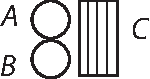
\includegraphics[width=0.15\textwidth]{%
gesamttex/edit_VIII,3/images/LH_37_05_155-156_d3_155v.pdf%
}} 
\vspace{0.5em}
\centerline{%
\lbrack\textit{Fig.~3}\rbrack%
}
% \newpage%
\vspace{1.em}
%
%
\pstart
Ponamus tria esse %
%
\edtext{corpor\lbrack a\rbrack}{\lemma{}\Bfootnote{corpore \textit{L ändert Hrsg.}}} mole aequalia\protect\index{Sachverzeichnis}{corpora mole aequalia}
%
\textit{A}.\textit{B}.\textit{C} duoque \textit{A}.\textit{B}.\ simul %
%
\edtext{aequivelociter}{\lemma{}\Bfootnote{aequivelociter \textit{erg.~L}}} 
%
parallele atque ita incurrere in \textit{C}, ut aeque ab ejus centro gravitatis\protect\index{Sachverzeichnis}{centrum gravitatis} absint, quo aequalem ambo ictum infligant. %
%
\edtext{Primum cogitemus,}{\lemma{Primum}\Bfootnote{\textit{(1)}~manifestum est \textit{(2)}~cogitemus,~\textit{L}}}
%
utrumquodque ex ipsis \textit{A}, et \textit{B}.\ dare celeritatem suam corpori \textit{C}, ergo corpus \textit{C} accepit potentiam\protect\index{Sachverzeichnis}{potentia} corporum \textit{A}.\textit{B}. 
%
Vicissim corpus \textit{C} dat corpori \textit{A} dimidiam et \textit{B} alteram dimidiam celeritatem, 
%
atque ita rursus prodit permutatio potentiarum\protect\index{Sachverzeichnis}{permutatio potentiarum} 
%
et difficile erit 
%
\edtext{in aliorum Hypothesibus}{%
\lemma{in aliorum Hypothesibus}%
\Cfootnote{%
Möglicherweise sind solche Autoren gemeint, deren Stoßregeln die Annahme der \glqq permutatio potentiarum\grqq\ nicht zulassen, wie bspw.\ \protect\index{Namensregister}{\textso{Huygens} (Hugenius, Ugenius, Hugens, Huguens), Christiaan 1629-1695}Huygens 
%
(\protect\vphantom)\cite{00529}\glqq Regles du mouvement dans la rencontre des corps\grqq, \cite{00157}\textit{JS}, Pariser Ausgabe, 18.~März 1669, S.~22\textendash24\protect\vphantom() und \protect\index{Namensregister}{\textso{Mariotte}, Edme, Seigneur de Chazeuil ca. 1620-1684}
Mariotte (\cite{00311}\textit{Traité de la percussion}, Paris 1673).}}
%
explicare tales casus. \pend
% %
\pstart 
\hspace{1mm}\hspace{-1mm}% Trick, weil \edlabel nicht zu \par-Beginn sein darf
\edlabel{37_05_155-156_9a}%	zwecks Referenzierung
Experiamur ratiocinationem per compositiones motuum,\protect\index{Sachverzeichnis}{ratiocinatio per compositiones motuum} eo casu quo id permissum est, neque potentiam\protect\index{Sachverzeichnis}{potentia} tollit.%
\edtext{}{%	% Trick Fig. 4
\lemma{\hspace*{1,6mm}%
\lbrack\textit{Fig.~4}\rbrack%
}\killnumber%
\Cfootnote{%
Ein gestrichener Entwurf zum Diagramm wird nicht wiedergegeben.%
}}
\pend
%
%
\vspace{1.0em} %%%%%%%%% Diagramm 4, gestr.
\centerline{%
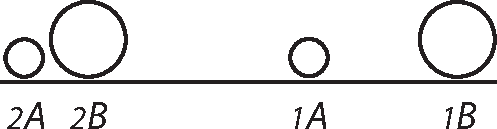
\includegraphics[width=0.3\textwidth]{%
gesamttex/edit_VIII,3/images/LH_37_05_155-156_d4_155v.pdf%
}} 
\vspace{0.5em}
\centerline{%
\lbrack\textit{Fig.~4, gestr.}\rbrack%
}
% \newpage%
\vspace{1em}
% %
\pstart 
Primum si 
%
\edtext{corpus incurrat}{%
\lemma{}%
\Bfootnote{%
corpus \textbar\ majus \textit{streicht Hrsg.}~\textbar\ incurrat~\textit{L}}}
%
in quiescens aequale,\protect\index{Sachverzeichnis}{incursus corporis in quiescens aequale} in ejus loco manebit\lbrack,\rbrack\ 
%
ipsum vero ante quiescens propellet. Quid ergo si sit majus, %
%
\edtext{tunc}{\lemma{}\Bfootnote{tunc \textit{erg.~L}}} 
%
 utique vel sequetur vel fortius propellet. Quid ergo si dicamus superfluam potentiam\protect\index{Sachverzeichnis}{potentia superflua} aequaliter ita inter utrumque distribui, ut ea ambo %
%
\edtext{praeterea eant,}{\lemma{praeterea}\Bfootnote{\textit{(1)}~sequantur \textit{(2)}~eant,~\textit{L}}}
%
 sive ut distribuatur inter corpora pro reciproca eorum %
%
\edtext{ratione. Sed si}{\lemma{ratione.}\Bfootnote{\textit{(1)}~Idque sic poterimus primum considerare: si corpus concurrant reciproca celeritate, ambo \textit{(2)}~Sed si~\textit{L}}}
%
 haec regula haberet locum, %
%
\edtext{tunc etiam corpore in quiescens aequale incurrente,\protect\index{Sachverzeichnis}{incursus corporis in quiescens aequale} videtur}{\lemma{tunc}\Bfootnote{\textit{(1)}~deberent \textit{(2)}~etiam corpore \textit{(a)}~uno \textit{(aa)}~aliud \textit{(bb)}~in aliud impingente deberent \textit{(b)}~in quiescens \textbar\ aequale \textit{erg.} \textbar\  incurrente, \textit{(aa)}~videntur ambo \textit{(bb)}~videtur~\textit{L}}}
%
 potentia\protect\index{Sachverzeichnis}{potentia} ipsis ita esse distribuenda, ut %
%
\edtext{pergant simul}{\lemma{pergant}\Bfootnote{\textit{(1)}~celeritate eadem sed in ratione \textit{(2)}~po \textit{(3)}~simul~\textit{L}}}
%
potentia\protect\index{Sachverzeichnis}{potentia} eadem. Quod si corpus quiescens excipiens\protect\index{Sachverzeichnis}{corpus quiescens excipiens} sit minus, %
%
\edtext{procedet celerior,}{\lemma{procedet}\Bfootnote{\textit{(1)}~tardius \textit{(2)}~celerior,~\textit{L}}}
%
sed hic difficultas, nam quid si sit majus procedet tardius quod fieri non potest. Itaque ubique difficultates. \pend
% %
\pstart 
\hspace{1mm}\hspace{-1mm}% Trick, weil \edlabel nicht zu \par-Beginn sein darf
\edlabel{37_05_155-156_10a}%
Videntur admittendae motuum compositiones\protect\index{Sachverzeichnis}{compositio motuum} cum potentiam non mutant, itaque videtur recte sic procedi %
%
\edtext{posse, cum}{\lemma{posse,}\Bfootnote{\textit{(1)}~praeter \textit{(2)}~cum~\textit{L}}}
%
corpus unum aliud assequitur, potest supponi rem fieri in navi,\protect\index{Sachverzeichnis}{navis} 
%
quae movetur motu praecedentis, sequens vero movebitur motuum differentia. 
%
\edtext{Et post ictum, navi\protect\index{Sachverzeichnis}{navis} %
%
\edtext{procedente, movebuntur}{\lemma{procedente,}\Bfootnote{\textit{(1)}~movebitur \textit{(2)}~movebuntur~\textit{L}}}
%
in navi\protect\index{Sachverzeichnis}{navis} corpora, 
%
ut alias determinatum supponitur fieri,}{%
\lemma{Et \lbrack...\rbrack\ fieri}%
\Cfootnote{%
Siehe N.~\ref{RK57269} vom 10.\ (20.) Juni 1677.}}
%
si motum in %
%
\edtext{quiescens incurrat. Porro si corpus motum incurrat}{\lemma{quiescens}\Bfootnote{incurrat. \textit{(1)}~De qui \textit{(2)}~Porro si corpus \textit{(a)}~incurrit \textit{(b)}~motum incurrat~\textit{L}}}
%
in quiescens invenio per motuum compositiones salva potentia\protect\index{Sachverzeichnis}{compositio motuum salva potentia} corpus %
%
\edtext{incurrens tempore}{\lemma{incurrens}\Bfootnote{\textit{(1)}~moveri differentia celeritatum per \textit{(2)}~tempore~\textit{L}}}
%
eodem quo accessit, percurrere differentiam distantiarum corporum a centro gravitatis\protect\index{Sachverzeichnis}{distantiae corporum a centro gravitatis} $\pleibdashv al\;\pleibvdash bl$, et %
%
\edtext{quidem reflecti}{\lemma{quidem}\Bfootnote{\textit{(1)}~reflecti si minus \textit{(2)}~pergere si \textit{(3)}~reflecti~\textit{L}}}
%
si major est distantia ejus corporis quod incurrit, a centro gravitatis,\protect\index{Sachverzeichnis}{centrum gravitatis}
%
seu si illud corpus minus est, pergere si majus. Alterum autem corpus nempe %
%
\edtext{excipiens\protect\index{Sachverzeichnis}{corpus excipiens} percurret eodem}{\lemma{excipiens}\Bfootnote{\textit{(1)}~movebitur eo \textit{(2)}~percurret eodem~\textit{L}}}
%
tempore duplicatam sui distantiam ab eodem centro gravitatis\protect\index{Sachverzeichnis}{centrum gravitatis} primo.%
\edlabel{37_05_155-156_10b}
\pend
%
\newpage
%
\vspace{1.2em} %%%%%%%%% Diagramm 5
\centerline{%
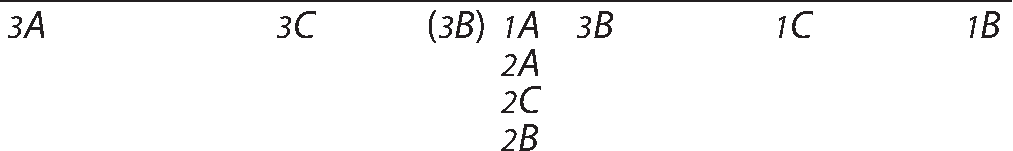
\includegraphics[width=0.75\textwidth]{%
gesamttex/edit_VIII,3/images/LH_37_05_155-156_d5_155v.pdf%
}} 
\vspace{0.5em}
\centerline{%
\lbrack\textit{Fig.~5}\rbrack%
}
% \newpage%
\vspace{1em}
%
%
\pstart 
${\scriptstyle \textit{1}}B{\scriptstyle \textit{1}}C \sqcap al$. ${\scriptstyle \textit{1}}A{\scriptstyle \textit{1}}C \sqcap bl$. 
${\scriptstyle \textit{1}}B{\scriptstyle \textit{2}}B \sqcap al+bl$. 
%
${\scriptstyle \textit{1}}C{\scriptstyle \textit{2}}C \sqcap {\scriptstyle \textit{2}}C{\scriptstyle \textit{3}}C \sqcap bl %
\edtext{\sqcap\, {\scriptstyle \textit{3}}C{\scriptstyle \textit{2}}B$.}{%
\lemma{}%
\Bfootnote{%
$\sqcap {\scriptstyle \textit{3}}C{\scriptstyle \textit{2}}B$ 
\textit{erg.~L}%
}}
%
${\scriptstyle \textit{3}}C{\scriptstyle \textit{3}}A \sqcap {\scriptstyle \textit{1}}C{\scriptstyle \textit{1}}A \sqcap bl$. 
${\scriptstyle \textit{3}}B{\scriptstyle \textit{3}}C \sqcap {\scriptstyle \textit{1}}B{\scriptstyle \textit{1}}C \sqcap al$.
\rule[0cm]{0mm}{14pt}${\scriptstyle \textit{2}}A{\scriptstyle \textit{3}}A \,\sqcap 
\begin{array}[t]{c} {\scriptstyle \textit{2}}C{\scriptstyle \textit{3}}C \\ bl \end{array} 
+ \begin{array}[t]{c} {\scriptstyle \textit{3}}C{\scriptstyle \textit{3}}A \\ bl \end{array} 
\sqcap 2bl$.
${\scriptstyle \textit{2}}B{\scriptstyle \textit{3}}B \,\sqcap 
\begin{array}[t]{c} \pleibdashv {\scriptstyle \textit{3}}B{\scriptstyle \textit{3}}C \\ \pleibdashv\, al \end{array}
\begin{array}[t]{c} \pleibvdash {\scriptstyle \textit{3}}C{\scriptstyle \textit{2}}B \\ \pleibvdash\, bl \end{array}$
%
ubi potentia\protect\index{Sachverzeichnis}{potentia} manet %
%
\edtext{eadem et}{\lemma{eadem}\Bfootnote{\textit{(1)}~eritque \textit{(2)}~et~\textit{L}}}
%
 corpus \textit{B} 
%
\edtext{reflecte\lbrack tur\rbrack}{%
\lemma{}%
\Bfootnote{%
reflectet %
\textit{L ändert Hrsg.}%
}}
%
 si \textit{al} sit major perget si \textit{bl}. \pend
%
%
\pstart
\lbrack156~r\textsuperscript{o}\rbrack\ Ergo si corpus aliud %
%
\edtext{assequatur tunc}{\lemma{assequatur}\Bfootnote{\textit{(1)}~post ictum corpus \textit{(2)}~tunc~\textit{L}}} %
%
ponendo celeritatem
%
$\overset{\displaystyle B}{\text{assequentis}}$ esse $al+bl+h$.\ scilicet \textit{h} existente celeritate %
%
\edtext{ipsius corporis}{\lemma{ipsius}\Bfootnote{\textit{(1)}~minoris \textit{(2)}~corporis~\textit{L}}} %
%
\rule[0cm]{0mm}{18pt}$\overset{\displaystyle A}{\text{praecedentis}}$, erit post ictum celeritas ipsius 
\rule[0cm]{0mm}{18pt}$\overset{\displaystyle B}{\text{assequentis}}$ %
%
\edtext{$\sqcap\;\pleibdashv al\,  \pleibvdash bl + h$.\ ubi notandum $\pleibdashv\; al \;\pleibvdash\; bl$ esse}%
{\lemma{$\sqcap\;\pleibdashv al\,  \pleibvdash bl + h$.}%
\Bfootnote{\textit{(1)}~at celeritas ipsius praecedentis \textit{(2)}~ubi notandum \textit{(a)}~redire si \textit{al} \textit{(b)}~\textbar\ si \textit{streicht Hrsg.}~\textbar\ $\pleibdashv\; al \;\pleibvdash\; bl$ sit quantitas affirmativa, ita \textit{(c)}~\textbar\ $\pleibdashv\; al \;\pleibvdash\; bl$ esse~\textit{L}}}
%
semper quantitatem affirmativam,\protect\index{Sachverzeichnis}{quantitas affirmativa} seu horum duorum differentiam, si %
%
\edtext{ergo \textit{bl} sit major quam \textit{al}, quo casu}{\lemma{ergo}\Bfootnote{\textit{(1)}~\textit{bl} sit minor quam \textit{al}, et \textit{(2)}~\textit{bl} sit \textit{(a)}~minor \textit{(b)}~major quam \textit{al}, \textit{(aa)}~et praeterea \textit{(bb)}~quo casu~\textit{L}}} %
%
 corpus incurrens non %
%
\edtext{reflectitur, tunc}{\lemma{reflectitur,}\Bfootnote{\textit{(1)}~et praeterea \textit{(2)}~tunc~\textit{L}}}
%
 corpus incurrens\protect\index{Sachverzeichnis}{corpus incurrens} \edtext{\textit{B},}{%
\lemma{}%
\Bfootnote{%
\textit{B} %
\textit{erg.~L}%
}}
%
quod  %
%
\edtext{scilicet est majus}{\lemma{scilicet est}\Bfootnote{\textit{(1)}~minus \textit{(2)}~majus~\textit{L}}}
%
excipiente, ibit celeritate $+bl-al+h$, et corpus excipiens\protect\index{Sachverzeichnis}{corpus excipiens} 
%
\edtext{\textit{A}}{%
\lemma{}%
\Bfootnote{%
\textit{A} %
\textit{erg.~L}%
}}
%
celeritate $2bl+h$. \pend
% %
\pstart Examinemus quod sit futurum, si duo corpora concurrant reciproca celeritate,\protect\index{Sachverzeichnis}{celeritates reciprocae}
%
ex iis ducendo consequentiam, quae fiunt uno quiescente. \pend
% %
\pstart Sint duo corpora \textit{a}.\textit{b}. celeritates \textit{e}.\textit{f}. et %
%
$ae \sqcap bf$. 
%
\edlabel{37_05_155-156_11a}Volumus hoc exhibere, in navi,\protect\index{Sachverzeichnis}{navis} 
%
ita ut appareat unum \textit{b}, quiescere.
%
Dabimus ipsi navi\protect\index{Sachverzeichnis}{navis} celeritatem corporis \textit{a}, nempe \textit{e}, ita in navi\protect\index{Sachverzeichnis}{navis} apparebit quiescere, in ripa\protect\index{Sachverzeichnis}{ripa} apparebit moveri celeritate \textit{e}, ergo ut %
%
\edtext{corpus \textit{B} celeritate}{\lemma{corpus \textit{B}}\Bfootnote{\textit{(1)}~moveatur \textit{(2)}~in l \textit{(3)}~celeritate~\textit{L}}}
%
\textit{f} moveri appareat spectanti e ripa,\protect\index{Sachverzeichnis}{ripa}\protect\index{Sachverzeichnis}{spectans e ripa} 
%
necesse est in navi\protect\index{Sachverzeichnis}{navis} moveri celeritate $f+e$, ut scilicet celeritas \textit{e}, ipsius %
%
\edtext{navis\protect\index{Sachverzeichnis}{navis} in}{\lemma{navis}\Bfootnote{\textit{(1)}~nihil \textit{(2)}~in~\textit{L}}}
%
contrarium\lbrack,\rbrack\ nihil ab apparentia\protect\index{Sachverzeichnis}{apparentia} in ripa,\protect\index{Sachverzeichnis}{ripa} %
%
%
\edlabel{37_05_155-156_5a}%
\edtext{}{% 
{\xxref%
{37_05_155-156_5a}{37_05_155-156_5b}}%
\lemma{detrahat.}%
\Bfootnote{\textit{(1)}~Jam sint duo corpora: $\alpha$.$\beta$ \textit{(2)}~Jam~\textit{L}}}%
detrahat.%
\edlabel{37_05_155-156_11b}
\pend
%
\pstart
Jam%
\edlabel{37_05_155-156_5b}
%
in ipsa quidem navi\protect\index{Sachverzeichnis}{navis} ex praecedentibus corpus impingens\protect\index{Sachverzeichnis}{corpus impingens} \textit{B}, quod ponimus majus, feretur (ex dictis) post ictum celeritate $bl-al$, %
%
\edtext{cui si auferatur}{\lemma{cui}\Bfootnote{\textit{(1)}~addatur \textit{(2)}~si auferatur~\textit{L}}}
%
celeritas navis\protect\index{Sachverzeichnis}{navis} in contrarium nempe \textit{e}.\ feretur celeritate $bl-al-e$. Corpus autem excipiens\protect\index{Sachverzeichnis}{corpus excipiens} %
%
\edtext{\textit{A}}{\lemma{}\Bfootnote{\textit{A} \textit{erg.~L}}} 
%
 feretur
%
\edtext{celeritate $2bl-e$, unde 
ex iis quae aliunde scimus}{\lemma{celeritate $2bl-e$,}\Bfootnote{\textit{(1)}~\textbar\ et \textit{streicht Hrsg.}~\textbar\ \textit{(2)}~\textbar~unde ex iis quae aliunde scimus \textit{erg.}~\textbar\ et~\textit{L}}} 
%
%
necesse 
%
\edtext{esset $2bl-e$ esse $\sqcap\, e$ et $al+e-bl \sqcap f$ et}{\lemma{esset}%
\Bfootnote{\textit{(1)}~$2bl+e$ esse $\sqcap\, e$ \lbrack...\rbrack\ $\sqcap\, f$  quorum prius impossibile. Unde patet methodum per compositiones motuum contradicere sibi ipsi %
\textit{(2)}~$2bl-e$ \lbrack...\rbrack\ $\sqcap\, f$ et~\textit{L}}}
%
quia $al+bl \sqcap e+f$.\ et $ae \sqcap bf$.\ hinc $al \sqcap e+f-bl$.\ et rursus $al \sqcap \displaystyle\frac{bfl}{e}$\rule[-4mm]{0pt}{10mm}. Ergo $e^2+ef-ebl \sqcap bfl$, seu %
%
$e^2+ef\sqcap bfl+ebl$ seu
%
dividendo 
%
\edtext{per $e+f$.}{%
\lemma{}%
\Bfootnote{%
per \textbar\ seu \textit{streicht Hrsg.}~\textbar\ $e+f$.~\textit{L}%
}}
%
erit $e \sqcap bl$.\ Ergo $al \sqcap f$. Hinc in $2bl-e \sqcap e$, substituendo pro $2bl$ ejus valorem $2e$, 
%
patet hanc aequationem esse veram, item in $al+e-bl \sqcap f$.\ substituendo valores
%
pro \textit{bl} et \textit{al} fiet $f\,\ovalbox{\!$+e-e$} \sqcap f$ unde patet haec consentire.%
\edlabel{37_05_155-156_9b}
\pend
%
%
\vspace{2.0em} %%%%%%%%% Diagramm 6
\centerline{%
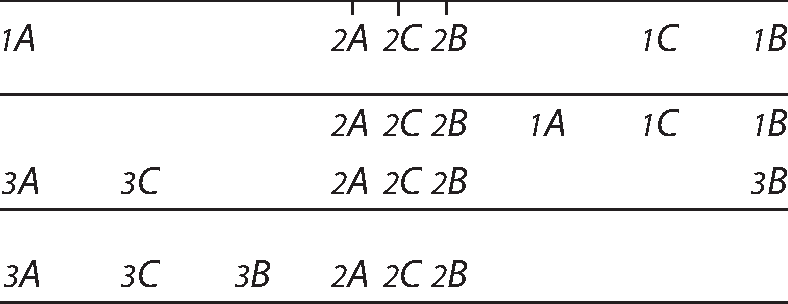
\includegraphics[width=0.58\textwidth]{%
gesamttex/edit_VIII,3/images/LH_37_05_155-156_d6_156r.pdf%
}} 
\vspace{0.5em}
\centerline{%
\lbrack\textit{Fig.~6}\rbrack%
}
% \newpage%
\vspace{1.5em}
%
\pstart 
Via centri gravitatis:\protect\index{Sachverzeichnis}{via centri gravitatis}
%
\edtext{${\scriptstyle \textit{2}}A{\scriptstyle \textit{2}}B \sqcap g.$}{%
\lemma{}%
\Bfootnote{%
${\scriptstyle \textit{2}}A{\scriptstyle \textit{2}}B \sqcap g.$ %
\textit{erg.~L}%
}}
%
\begin{tabular}[t]{c}$f+g\;\pleibdashv e$\\${\scriptstyle \textit{1}}B{\scriptstyle \textit{2}}B+{\scriptstyle \textit{2}}B{\scriptstyle \textit{2}}A\;\pleibdashv {\scriptstyle \textit{2}}A{\scriptstyle \textit{1}}A$\end{tabular}
%
$\sqcap$ 
%
\begin{tabular}[t]{c}$bl+al$\phantom{\pleibdashv}\\${\scriptstyle \textit{1}}A{\scriptstyle \textit{1}}C+{\scriptstyle \textit{1}}C{\scriptstyle \textit{1}}B$\end{tabular},
%
\edlabel{37_05_155-156_6a}%
\edtext{}{% B-Footnote – Erg.
{\xxref%
{37_05_155-156_6a}{37_05_155-156_6b}}%
\lemma{}%
\Bfootnote{%
, si \lbrack...\rbrack\ 
$\protect\underset%
{\displaystyle \text{eodem tendent}}% Unten
{\text{occurrent}\protect\vphantom{j}}$ % Mittig
\textit{erg.~L}%
}}%
si \pleibdashv est %
\begin{tabular}[t]{c}$+$\\$-$\end{tabular} %
corpora %
\begin{tabular}[t]{c}occurrent\\eodem tendent\end{tabular}.%
\edlabel{37_05_155-156_6b}
%
%
\edtext{Ergo $g \sqcap bl+al-f\; \pleibvdash e$.}{%
\lemma{}%
\Bfootnote{%
Ergo $g \sqcap bl+al-f\; \pleibvdash e$. %
\textit{erg.~L}%
}}
%
%
\pend
%
\pstart
\rule[0cm]{0mm}{11pt}${\scriptstyle \textit{1}}C{\scriptstyle \textit{2}}C\; \sqcap$%
$\begin{array}[t]{r}{\scriptstyle \textit{1}}C{\scriptstyle \textit{1}}A\\bl\end{array}%
\raisebox{-0.4em}{\pleibvdash}\!%
\begin{array}[t]{l}{\scriptstyle \textit{1}}A{\scriptstyle \textit{2}}A\\e\end{array}%
-{\scriptstyle \textit{2}}A{\scriptstyle \textit{2}}C \,\sqcap\, -{\scriptstyle \textit{1}}C{\scriptstyle \textit{1}}B+{\scriptstyle \textit{1}}B{\scriptstyle \textit{2}}B+{\scriptstyle \textit{2}}B{\scriptstyle \textit{2}}C$.%
\pend
%
\pstart
%
\edtext{$\displaystyle\frac{{\scriptstyle \textit{1}}B{\scriptstyle \textit{2}}C}{{\scriptstyle \textit{1}}B{\scriptstyle \textit{1}}C} \sqcap \displaystyle\frac{{\scriptstyle \textit{2}}A{\scriptstyle \textit{2}}C}{{\scriptstyle \textit{1}}A{\scriptstyle \textit{1}}C} \sqcap \displaystyle\frac{g \sqcap bl+al-f\;\leibvdash\; e}{bl+al}$. Ergo ${\scriptstyle \textit{2}}A{\scriptstyle \textit{2}}C \sqcap \displaystyle\frac{\overline{bl}^2+albl-fbl\;\leibvdash\; ebl}{bl+al} \sqcap bl-\displaystyle\frac{+f\;\leibdashv\; e}{bl+al}bl$.}{%
\lemma{$\displaystyle\frac{{\scriptstyle \textit{1}}B{\scriptstyle \textit{2}}C}{{\scriptstyle \textit{1}}B{\scriptstyle \textit{1}}C}$}%
\Bfootnote{%
\lbrack...\rbrack\ $- \displaystyle\frac{+f\;\leibdashv\; e}{bl+al}bl$. %
\textit{erg.~L}%
}}
%
\pend
%
\pstart
\rule[0cm]{0mm}{20pt}Ergo ${\scriptstyle \textit{1}}C{\scriptstyle \textit{2}}C \sqcap \ovalbox{\textit{bl}}\; \pleibvdash e\;\ovalbox{$-bl$}+\displaystyle\frac{f\;\leibdashv\; e}{bl+al}bl$ seu $\displaystyle\frac{\ovalbox{$\leibvdash ble$}\;\leibvdash\; ale+blf\, \ovalbox{$\leibdashv ble$}}{bl+al} \sqcap \displaystyle\frac{+bf\; \leibvdash\; ae}{b+a}$\rule[-4mm]{0pt}{12mm} %
%
\edtext{id est eadem}{\lemma{id est}\Bfootnote{\textit{(1)}~via centri erit summa utri \textit{(2)}~eadem~\textit{L}}}
%
\rule[0cm]{0mm}{10pt}est potentia\protect\index{Sachverzeichnis}{potentia} corporum via centri\protect\index{Sachverzeichnis}{via centri gravitatis} incedentium, 
%
quae est differentia potentiarum\protect\index{Sachverzeichnis}{differentia potentiarum} si sibi occurrunt, 
%
et quae est summa\protect\index{Sachverzeichnis}{summa potentiarum} si se sequuntur. 
%
Quod si corpora divergant, idem est ac si occurrant. 
%
Porro post occursum\protect\index{Sachverzeichnis}{occursus} celeritates sunt \textit{i} et \textit{m}.\ et quemadmodum ante concursum\protect\index{Sachverzeichnis}{concursus} 
%
unum ex corporibus semper sequitur centrum gravitatis,\protect\index{Sachverzeichnis}{centrum gravitatis}
%
ita post concursum\protect\index{Sachverzeichnis}{concursus} unum semper praecedit, ponendo id in easdem ire partes. 
%
Invertamus autem omnia et faciamus quasi ex loco quo post ictum\protect\index{Sachverzeichnis}{ictus} 
%
pervenere corpora redirent ad locum ictus,\protect\index{Sachverzeichnis}{ictus}
%
patet eo casu calculando viam centri\protect\index{Sachverzeichnis}{via centri gravitatis} 
%
quod etiam redire in locum ictus\protect\index{Sachverzeichnis}{ictus}
%
(ex \textit{{\scriptsize3}C} ad \textit{{\scriptsize2}C}) intelligitur corpus \textit{A} nunc necessario sequi 
%
centrum, cum antea id quod sequebatur esset \textit{B}. 
%
Ergo ${\scriptstyle \textit{3}}C{\scriptstyle \textit{2}}C \sqcap \displaystyle\frac{ai(\leibvdash)bm}{a+b}$\rule[-4mm]{0pt}{10mm}. %
%
\edtext{Cumque sit}{\lemma{Cumque}\Bfootnote{\textit{(1)}~sint \textit{(2)}~sit~\textit{L}}}
%
 ${\scriptstyle \textit{3}}C{\scriptstyle \textit{2}}C \sqcap {\scriptstyle \textit{1}}C{\scriptstyle \textit{2}}C$ erit $bf\pleibvdash ae \sqcap ai (\pleibvdash) bm$. 
%
Jam ex natura manentis potentiae\protect\index{Sachverzeichnis}{potentia} debet esse $ae+bf \sqcap ai+bm$. \pend
%
%
\pstart 
%
\lbrack156~v\textsuperscript{o}\rbrack\ 
%
Videamus ergo quid ex his duabus aequationibus junctis: 
%
$ae+bf \sqcap ai+bm$. et $\pleibvdash ae + bf \sqcap ai (\pleibvdash) bm$ 
%
duci possit.%
\pend
%
\pstart\noindent
$bf-ai \sqcap bm-ae$ ex priore, et $bf-ai \,\sqcap\; \pleibdashv\; ae (\pleibvdash) bm$. %
\pend
%
\pstart\noindent
Ergo $bm-ae \,\sqcap\, \pleibdashv\, ae (\pleibvdash) bm$. Ubi si corpora se sequantur fiet $bm\,\ovalbox{\!$-ae$} \,\sqcap \,\ovalbox{\!$-ae$}\, (\pleibvdash) bm$. Ergo si corpora se sequantur, fit necessario $(\pleibvdash) \sqcap +$ seu $(\pleibdashv) \sqcap -$. %
\pend
%
\pstart\noindent
Id est si corpora se 
%
\edtext{sequantur, necessario sequentur post ictum.\protect\index{Sachverzeichnis}{ictus}}{%
\lemma{sequantur,}%
\Bfootnote{%
\textit{(1)}~\textbar\ post ictum \textit{streicht Hrsg.}~\textbar\ necessario divergent, (\protect\vphantom)quod non videtur consentire cum compositione ex motu in navi, ubi sane manifestum est, si impingat in navi motum in quiescens minus pergere, quod examinandum et cum calculo in navi conferendum.\protect\vphantom()
\textit{(2)}~necessario sequentur post ictum.~\textit{L}%
}}
%
%
Si corpora sibi occurrant erit $bm-ae \sqcap +ae (\pleibvdash) bm$. Ergo $2ae \sqcap bm (\pleibdashv) bm$. %
%
\edtext{Ubi necessario}{\lemma{Ubi}\Bfootnote{\textit{(1)}~cum \textit{e} sit \textit{(2)}~necessario~\textit{L}}}
%
erit $(\pleibdashv) \sqcap +$. Seu %
%
\edtext{$\xout{2}ae \sqcap \xout{2}bm$ excepto}{\lemma{$\xout{2}ae \sqcap \xout{2}bm$}\Bfootnote{\textit{(1)}~. Si scilicet \textit{(2)}~excepto~\textit{L}}}
%
 uno casu, ubi $e \sqcap 0$.\ seu ubi corpus \textit{A} quiescere ante ictum intelligitur, tunc enim duo hinc sequuntur, vel corpus \textit{B}, etiam quiescere post ictum\protect\index{Sachverzeichnis}{ictus}
%
seu $m \sqcap 0$. Hinc potest fieri $(\pleibdashv)\sqcap +$, vel possumus assumere
%
 $(\pleibdashv)\sqcap -$. Tunc fiet $2ae \sqcap 0$. Quod jam novimus, 
%
et tantum inde sequitur corpora post ictum\protect\index{Sachverzeichnis}{ictus} divergere. Ergo %
%
\edtext{ex combinatione}{\lemma{ex}\Bfootnote{\textit{(1)}~hoc theorem \textit{(2)}~combinatione~\textit{L}}}
%
harum duarum regularum de servata potentia,\protect\index{Sachverzeichnis}{potentia}\protect\index{Sachverzeichnis}{regula de servata potentia} et de celeritate %
%
\edtext{centri\protect\index{Sachverzeichnis}{centrum gravitatis} et directione eadem, %
\protect\index{Sachverzeichnis}{regula de eadem celeritate et directione centri gravitatis} %
hoc}%
{\lemma{centri}%
\Bfootnote{\textit{(1)}~, hoc unum constans \textit{(2)}~et directione eadem, \textit{(a)}~hoc unum certo colligimus, quod \textit{(b)}~hoc~\textit{L}}}
%
tantum certo colligimus: %
\pend
%
\pstart
\hspace{1mm}\hspace{-1mm}% Trick, weil \edlabel nicht zu \par-Beginn sein darf
\edlabel{37_05_155-156_7a}%
1.\ Si corpora se sequuntur  %
%
\edtext{ante ictum\protect\index{Sachverzeichnis}{ictus} se sequentur}{\lemma{ante ictum}\Bfootnote{\textit{(1)}~divergent \textit{(2)}~se sequentur~\textit{L}}}
%
post ictum.\protect\index{Sachverzeichnis}{ictus}%
\pend
%
\pstart
2.\ Si %
%
\edtext{corpora sibi occurrant ante}{\lemma{corpora}\Bfootnote{\textit{(1)}~ambo sint in motu et sib \textit{(2)}~sibi occurrant \textit{(a)}~tunc \textit{(b)}~ante~\textit{L}}}
%
ictum,\protect\index{Sachverzeichnis}{ictus} divergent post ictum\protect\index{Sachverzeichnis}{ictus}
%
permutatis potentiis.\protect\index{Sachverzeichnis}{permutatio potentiarum}%
\pend
%
\pstart
3.\ Si corpus incurrat in aliud quiescens,\protect\index{Sachverzeichnis}{incursus corporis in aliud quiescens} tunc vel corpus incurrens\protect\index{Sachverzeichnis}{corpus incurrens} etiam quiescet post ictum,\protect\index{Sachverzeichnis}{ictus} vel ambo se sequentur. %
\pend
%
\pstart
4.\ Si ponantur permutari potentiae\protect\index{Sachverzeichnis}{permutatio potentiarum} %
et directiones\protect\index{Sachverzeichnis}{permutatio directionum} %
per ictum,\protect\index{Sachverzeichnis}{ictus} %
tunc simul observabitur utraque regula scilicet %
conservatio potentiae corporum,\protect\index{Sachverzeichnis}{conservatio potentiae corporum} %
et directionis centri.\protect\index{Sachverzeichnis}{conservatio directionis centri}\edlabel{37_05_155-156_7b}
%
\pend
%
\pstart
Quoniam si corpora sibi occurrant necessario fit $+ae+bf \sqcap ai+bm$. Hinc patet hinc nihil detegi novi nec absolvi problema ex his duabus regulis. %
\pend
%
\pstart
Si corpus \textit{e} quiescat, fit: $bf \sqcap ai\; \pleibvdash bm$. Ergo si $m \sqcap 0$. necessario $bf \sqcap ai$. Sed si ponamus se sequi corpora post ictum\protect\index{Sachverzeichnis}{ictus} et esse $bf \sqcap ai+bm$, rursus nihil hinc novi ducemus de modo scilicet, quo se corpora sequi debeant. \pend
% %
\pstart 
Si 
%
\edtext{finxissemus centrum}{%
\lemma{finxissemus}%
\Bfootnote{%
\textit{(1)}~corpus %
\textit{(2)}~centrum~\textit{L}%
}}
%
gravitatis\protect\index{Sachverzeichnis}{centrum gravitatis} post ictum eadem qua venerat celeritate redire, fieret aequatio: $\pleibvdash\; ae+bf \sqcap (\pleibvdash) ai+bm$.\
%
et fieret $bf-bm \sqcap (\pleibvdash) ai \;\pleibdashv\; ae$ at idem %
%
\edtext{$bf-bm \sqcap ai-ae$. Ergo}{\lemma{$bf-bm \sqcap ai-ae$.}\Bfootnote{\textit{(1)}~Quae aequatio esset \textit{(2)}~Ergo~\textit{L}}}
%
 $ai-ae \sqcap (\pleibvdash) ai \;\pleibdashv\; ae$.\ seu $i-e \sqcap (\pleibvdash) i \;\pleibdashv\; e$.
%
Quod si %
%
\edtext{corpora sibi}{\lemma{corpora}\Bfootnote{\textit{(1)}~sequantur, res est absurda \textit{(2)}~sibi~\textit{L}}}
%
occurrant ante ictum\protect\index{Sachverzeichnis}{ictus}\lbrack,\rbrack\ fiet $i-e \sqcap (\pleibvdash) i+e$. seu $2e \sqcap +i (\pleibdashv) i$, id est vel $2e \sqcap 2i$ quod absurdum est, nisi ambo sint aequalia et aequali celeritate %
%
\edtext{ferantur, et}{\lemma{ferantur,}\Bfootnote{\textit{(1)}~vel erit \textit{(2)}~et~\textit{L}}}
%
ita post ictum\protect\index{Sachverzeichnis}{ictus} divergent, vel $2e \sqcap 0$.\ quod est absurdum. 
%
Ergo si corpora sibi occurrant regula de recursu centri gravitatis\protect\index{Sachverzeichnis}{regula de recursu centri gravitatis} 
%
servari non potest nisi in casu, quo vel centrum\protect\index{Sachverzeichnis}{centrum gravitatis} ipsum quiescit, seu ejus recursus infinite parvus,
%
vel in casu quo corpus unum alteri celeritate infinite parva\protect\index{Sachverzeichnis}{celeritas infinite parva} occurit seu quiescit. 
%
Si corpora se sequantur, tunc fiet $i-e \sqcap (\pleibvdash) i-e$.\ seu $i \sqcap (\pleibvdash) i$ ergo $\pleibvdash\; \sqcap\; +$ seu $\pleibdashv\; \sqcap\; -$ 
%
seu corpora se sequentur etiam post ictum in contrariam partem, quae omnia absurda: 
%
absurdum ergo centrum gravitatis\protect\index{Sachverzeichnis}{centrum gravitatis} eadem celeritate qua venit sic redire. \pend
\count\Afootins=1200%
\count\Bfootins=1200%
\count\Cfootins=1200